\documentclass{article}
\usepackage{amsthm,amsmath,amsfonts,amssymb,mathtools}
\usepackage[colorlinks,citecolor=blue,urlcolor=blue]{hyperref}
\usepackage{enumitem}
\usepackage[margin=1in]{geometry}

% Some useful macros.
\newcommand{\given}{\,|\,}
\newcommand{\trans}{\mathsf{T}}
\newcommand{\bx}{\mathbf{x}}
\newcommand{\by}{\mathbf{y}}
\newcommand{\bw}{\mathbf{w}}
\newcommand{\distNorm}{\mathcal{N}}
\newcommand{\bzero}{\mathbf{0}}
\newcommand{\btheta}{\boldsymbol{\theta}}
\newcommand{\bpi}{\boldsymbol{\pi}}
\newcommand{\ep}{\varepsilon}
\def\ie{i.e.\ }
\def\eg{e.g.\ }
\def\iid{i.i.d.\ }
\def\simiid{\sim_{\mbox{\tiny iid}}}
\newcommand{\varv}{\mathbb{V}}
\newcommand{\LL}[1]{\frac{\partial \log \pi(a_{#1}| s_{#1}, \theta)}{\partial \theta}}
\newcommand{\PT}{\frac{\partial}{\partial \theta}}
\newcommand{\PP}[1]{\frac{\partial}{\partial #1}}
\newcommand{\PPH}{\frac{\partial}{\partial \phi}}
\newcommand{\LP}[1]{\PT \log p(#1)}
\newcommand{\LZ}[1]{\frac{\log \pi(z_{#1}| s_{#1}, \theta)}{\partial \theta}}
\newcommand{\N}{\mathcal{N}}

\begin{document}
\title{Assignment 2:\\Stochastic Variational Inference in the TrueSkill Model}
\author{STA414/STA2014 and CSC412/CSC2506 Winter 2020\\
  \\
  (Bill) Yuan Liu\\
  Student Number: 996954078
}
\maketitle

Please see A2\_starter.jl for code.\\

The goal of this assignment is to get you familiar with the basics of
Bayesian inference in large models with continuous latent variables, and the basics of stochastic variational inference.

\paragraph{Background}
We'll implement a variant of the TrueSkill model, a player ranking system for competitive games originally developed for Halo 2.
It is a generalization of the Elo rating system in Chess.
For the curious, the original 2007 NIPS paper introducing the trueskill paper can be found here:
\url{http://papers.nips.cc/paper/3079-trueskilltm-a-bayesian-skill-rating-system.pdf}

This assignment is based on one developed by Carl Rasmussen at Cambridge for his course on probabilistic machine learning:
\url{http://mlg.eng.cam.ac.uk/teaching/4f13/1920/}


\subsection{Model definition}
We'll consider a slightly simplified version of the original trueskill model.
We assume that each player has a true, but unknown skill $z_i \in \mathbb{R}$.
We use $N$ to denote the number of players.

\paragraph{The prior.}
The prior over each player's skill is a standard normal distribution, and all player's skills are \emph{a prior} independent.  

\paragraph{The likelihood.}
For each observed game, the probability that player $i$ beats player $j$, given the player's skills $z_A$ and $z_B$, is:
$$p(\textnormal{A beat B} | z_A, z_B) = \sigma(z_i - z_j)$$
where
$$\sigma(y) = \frac{1}{1 + \exp(-y)}$$
There can be more than one game played between a pair of players, and in this case the outcome of each game is independent given the players' skills.
We use $M$ to denote the number of games.

\paragraph{The data.}
The data will be an array of game outcomes.
Each row contains a pair of player indices.
The first index in each pair is the winner of the game, the second index is the loser.
If there were $M$ games played, then the array has shape $M \times 2$.

\pagebreak
\section{Implementing the model [10 points]}
\begin{enumerate}[label=(\alph*)]
	\item {\bf [2 points]} Implement a function \texttt{log\_prior} that computes the log of the prior over all player's skills.
          Specifically, given a $K \times N$ array where each row is a setting of the skills for all $N$ players, it returns a $K \times 1$ array, where each row contains a scalar giving the log-prior for that set of skills.

\begin{verbatim}
function log_prior(zs)
  N = size(zs)[1]
  -1/2 * sum(zs.*zs,dims=1) .+ N*log(1/sqrt(2*pi))
end
\end{verbatim}
          
  \item {\bf [3 points]} Implement a function \texttt{logp\_a\_beats\_b} that, given a pair of skills $z_a$ and $z_b$
    evaluates the log-likelihood that player with skill $z_a$ beat player with skill $z_b$ under the model detailed above.
    To ensure numerical stability, use the function  \texttt{log1pexp} that computes $\log(1 + \exp(x))$ in a numerically stable way.
    This function is provided by \texttt{StatsFuns.jl} and imported already, and also by Python's numpy.

\begin{verbatim}
function logp_a_beats_b(za,zb)
  -log1pexp.(zb.-za)
end
\end{verbatim}
    
  \item {\bf [3 points]} Assuming all game outcomes are i.i.d. conditioned on all players' skills, implement a function \texttt{all\_games\_log\_likelihood} that takes a batch of player skills \texttt{zs} and a collection of observed games \texttt{games} and gives a batch of log-likelihoods for those observations.
  Specifically, given a $K \times N$ array where each row is a setting of the skills for all $N$ players, and an $M \times 2$ array of game outcomes, it returns a $K \times 1$ array, where each row contains a scalar giving the log-likelihood of all games for that set of skills.
  Hint: You should be able to write this function without using for loops, although you might want to start that way to make sure what you've written is correct.  If $A$ is an array of integers, you can index the corresponding entries of another matrix $B$ for every entry in $A$ by writing \texttt{B[A]}.

\begin{verbatim}
function all_games_log_likelihood(zs,games)
  zs_a = zs[games[:,1],:]
  zs_b =  zs[games[:,2],:]
  likelihoods =  logp_a_beats_b(zs_a,zs_b)
  sum(likelihoods,dims=1)
end
\end{verbatim}
  
\item {\bf [2 points]} Implement a function \texttt{joint\_log\_density} which combines the log-prior and log-likelihood of the observations to give $p(z_1, z_2, \dots, z_N, \text{all game outcomes})$

\begin{verbatim}
function joint_log_density(zs,games)
  all_games_log_likelihood(zs,games) .+ log_prior(zs)
end
\end{verbatim}
  
\pagebreak
  
\begin{verbatim}
@testset "Test shapes of batches for likelihoods" begin
  B = 15 # number of elements in batch
  N = 4 # Total Number of Players
  test_zs = randn(4,15)
  test_games = [1 2; 3 1; 4 2] # 1 beat 2, 3 beat 1, 4 beat 2
  @test size(test_zs) == (N,B)
  #batch of priors
  @test size(log_prior(test_zs)) == (1,B)
  # loglikelihood of p1 beat p2 for first sample in batch
  @test size(logp_a_beats_b(test_zs[1,1],test_zs[2,1])) == ()
  # loglikelihood of p1 beat p2 broadcasted over whole batch
  @test size(logp_a_beats_b.(test_zs[1,:],test_zs[2,:])) == (B,)
  # batch loglikelihood for evidence
  @test size(all_games_log_likelihood(test_zs,test_games)) == (1,B)
  # batch loglikelihood under joint of evidence and prior
  @test size(joint_log_density(test_zs,test_games)) == (1,B)
end
\end{verbatim}

\begin{figure}[h]
  \centering
  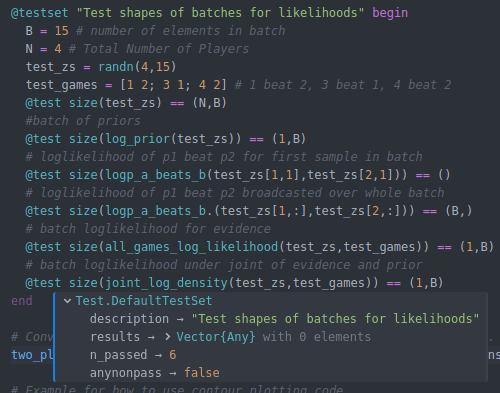
\includegraphics[width=12cm,keepaspectratio]{plots/testcase.png}
\end{figure}

\end{enumerate}

\pagebreak

\section{Examining the posterior for only two players and toy data [10 points]}
To get a feel for this model, we'll first consider the case where we only have 2 players, $A$ and $B$.
We'll examine how the prior and likelihood interact when conditioning on different sets of games. 

Provided in the starter code is a function \texttt{skillcontour!} which evaluates a provided function on a grid of $z_A$ and $z_B$'s and plots the isocontours of that function.
As well there is a function \texttt{plot\_line\_equal\_skill!}. 
We have included an example for how you can use these functions.

We also provided a function \texttt{two\_player\_toy\_games} which produces toy data for two players.
I.e. \texttt{two\_player\_toy\_games(5,3)} produces a dataset where player A wins 5 games and player B wins 3 games.

\begin{enumerate}[label=(\alph*)]
\item {\bf [2 points]}  For two players $A$ and $B$, plot the isocontours of the joint prior over their skills.  Also plot the line of equal skill, $z_A = z_B$.
  Hint: you've already implemented the \textbf{log} of the likelihood function.

\begin{verbatim}
plot(title="Prior Contour Plot",
    xlabel = "Player 1 Skill",
    ylabel = "Player 2 Skill")
skillcontour!(zs -> exp(log_prior(zs)))
plot_line_equal_skill!()
savefig(joinpath("plots","prior_contour.png"))
\end{verbatim}

\begin{figure}[h]
  \centering
  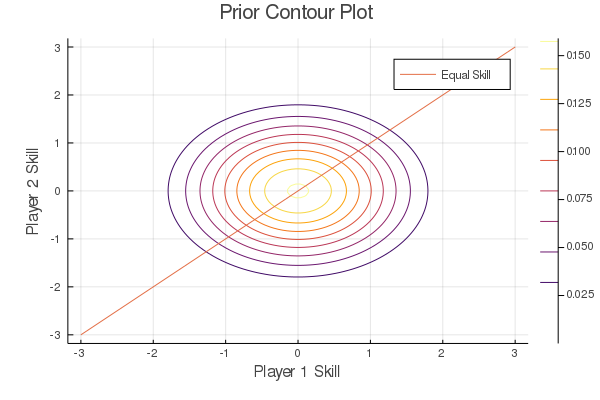
\includegraphics[width=12cm,keepaspectratio]{plots/prior_contour.png}
\end{figure}

\pagebreak

\item {\bf [2 points]} Plot the isocontours of the likelihood function. 
Also plot the line of equal skill, $z_A = z_B$.

\begin{verbatim}
plot(title="Likelihood Contour Plot",
    xlabel = "Player 1 Skill",
    ylabel = "Player 2 Skill")
skillcontour!(zs -> exp.(logp_a_beats_b(zs[1,:],zs[2,:])))
plot_line_equal_skill!()
savefig(joinpath("plots","likelihood_contour.png"))
\end{verbatim}

\begin{figure}[h]
  \centering
  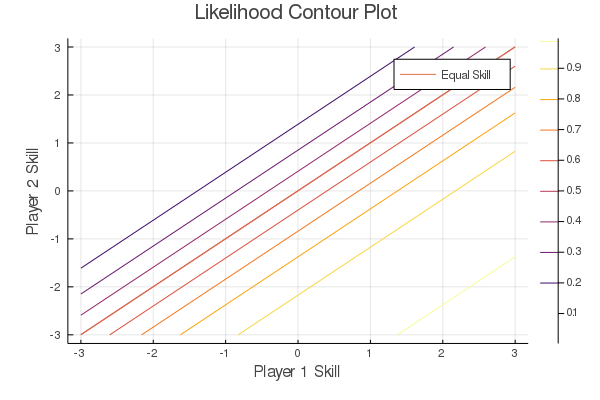
\includegraphics[width=12cm,keepaspectratio]{plots/likelihood_contour.png}
\end{figure}

\pagebreak

\item {\bf [2 points]}  Plot isocountours of the joint posterior over $z_A$ and $z_B$ given that player A
beat player B in one match.  Since the contours don't depend on the normalization
constant, you can simply plot the isocontours of the log of joint distribution of
$p(z_A, z_B, \text{A beat B})$
Also plot the line of equal skill, $z_A = z_B$.

\begin{verbatim}
games = two_player_toy_games(1,0)

plot(title="Joint Contour Plot, A Winning 1 Game",
    xlabel = "Player 1 Skill",
    ylabel = "Player 2 Skill")
skillcontour!(zs -> exp(joint_log_density(zs,games)))
plot_line_equal_skill!()
savefig(joinpath("plots","joint_contour_A1_B0.png"))
\end{verbatim}

\begin{figure}[h]
  \centering
  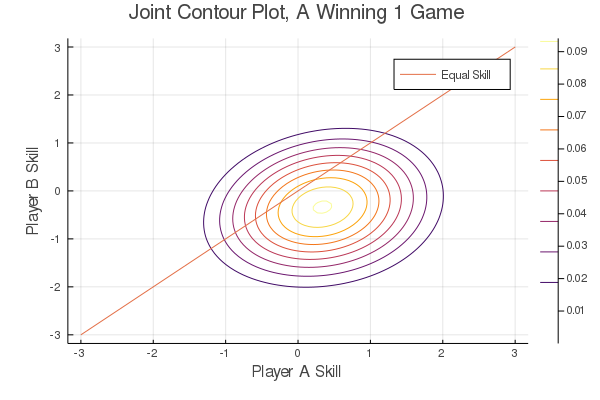
\includegraphics[width=12cm,keepaspectratio]{plots/joint_contour_A1_B0.png}
\end{figure}

\pagebreak

\item {\bf [2 points]}  Plot isocountours of the joint posterior over $z_A$ and $z_B$ given that
10 matches were played, and player A beat player B all 10 times.
Also plot the line of equal skill, $z_A = z_B$.

\begin{verbatim}
games = two_player_toy_games(10,0)

plot(title="Joint Contour Plot, A Winning 10 Games",
    xlabel = "Player 1 Skill",
    ylabel = "Player 2 Skill")
skillcontour!(zs -> exp(joint_log_density(zs,games)))
plot_line_equal_skill!()
savefig(joinpath("plots","joint_contour_A10_B0.png"))
\end{verbatim}

\begin{figure}[h]
  \centering
  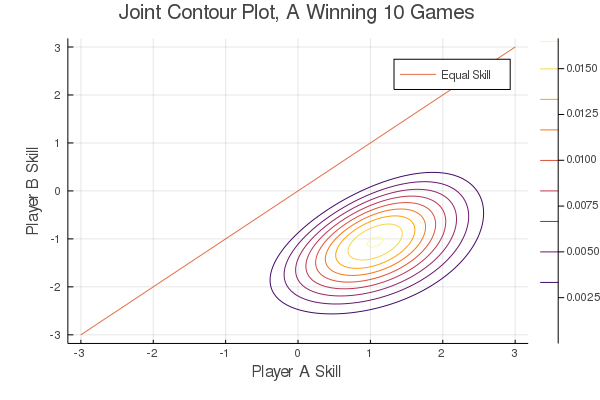
\includegraphics[width=12cm,keepaspectratio]{plots/joint_contour_A10_B0.png}
\end{figure}

\pagebreak

\item {\bf [2 points]}  Plot isocountours of the joint posterior over $z_A$ and $z_B$ given that
20 matches were played, and each player beat the other 10 times.
Also plot the line of equal skill, $z_A = z_B$.

\begin{verbatim}
games = two_player_toy_games(10,10)

plot(title="Joint Contour Plot, A Winning 10 Games, B Winning 10 Games",
    xlabel = "Player 1 Skill",
    ylabel = "Player 2 Skill")
skillcontour!(zs -> exp(joint_log_density(zs,games)))
plot_line_equal_skill!()
savefig(joinpath("plots","joint_contour_A10_B10.png"))
\end{verbatim}

\begin{figure}[h]
  \centering
  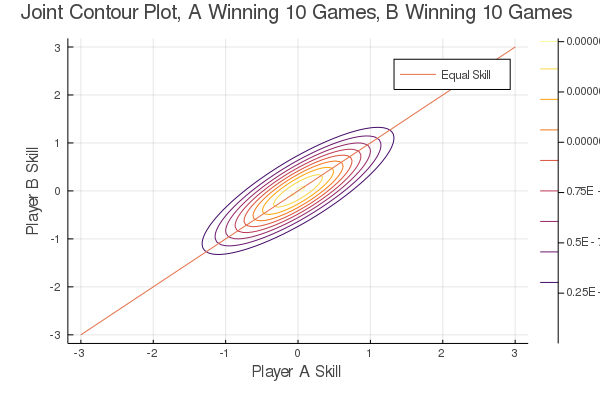
\includegraphics[width=12cm,keepaspectratio]{plots/joint_contour_A10_B10.png}
\end{figure}

\end{enumerate}

\pagebreak
\section{Stochastic Variational Inference on Two Players and Toy Data [18 points]}

One nice thing about a Bayesian approach is that it separates the model specification from the approximate inference strategy.
The original Trueskill paper from 2007 used message passing.
Carl Rasmussen's assignment uses Gibbs sampling, a form of Markov Chain Monte Carlo.
We'll use gradient-based stochastic variational inference, which wasn't invented until around 2014. 

In this question we will optimize an approximate posterior distribution with
stochastic variational inference to approximate the true posterior.

\begin{enumerate}[label=(\alph*)]
  \item {\bf [5 points]} Implement a function \texttt{elbo} which computes an unbiased estimate of 
    the evidence lower bound.
    As discussed in class, the ELBO is equal to the KL divergence between the true posterior $p(z|\text{data})$, and an approximate posterior, $q_\phi(z|\text{data})$, plus an unknown constant.
    Use a fully-factorized Gaussian distribution for $q_\phi(z|\text{data})$.
    This estimator takes the following arguments:
    \begin{itemize}
    	\item \texttt{params}, the parameters $\phi$ of the approximate posterior $q_\phi(z|\text{data})$.
    	\item A function \texttt{logp}, which is equal to the true posterior plus a constant.  This function must take a batch of samples of $z$.  If we have $N$ players, we can consider $B$-many samples from the joint over all players' skills.
    	This batch of samples \texttt{zs} will be an array with dimensions $(N,B)$.
    	\item \texttt{num\_samples}, the number of samples to take.
    \end{itemize}
    This function should return a single scalar.
    Hint: You will need to use the reparamterization trick when sampling \texttt{zs}.

\begin{verbatim}
function elbo(params,logp,num_samples)

  lsigma = params[2]
  sigma = exp.(params[2])
  m = params[1]

  N = length(params[1]) #number of players
  B = num_samples #batch size of samples

  s = randn(Float64, (N, B))
  samples = sigma .* s .+ m

  logp_estimate = logp(samples)
  logq_estimate = factorized_gaussian_log_density(m,lsigma,samples)

  mean((logp_estimate .- logq_estimate),dims=2)
end
\end{verbatim}
    
  \item {\bf [2 points]} Write a loss function called \texttt{neg\_toy\_elbo}
    that takes variational distribution parameters and an array of game outcomes, and returns the negative
    elbo estimate with 100 samples.

\begin{verbatim}
# Conveinence function for taking gradients
function neg_toy_elbo(params; games = two_player_toy_games(1,0), num_samples = 100)
  # TODO: Write a function that takes parameters for q,
  # evidence as an array of game outcomes,
  # and returns the -elbo estimate with num_samples many samples from q
  logp(zs) = joint_log_density(zs,games)
  return -elbo(params,logp, num_samples)
end
\end{verbatim}
    
  \item {\bf [5 points]} Write an optimization function called \texttt{fit\_toy\_variational\_dist}
    which takes initial variational parameters, and the evidence.
    Inside it will perform a number of iterations of gradient descent where for each iteration :
    \begin{enumerate}
      \item Compute the gradient of the loss with respect to the parameters using automatic differentiation.
      \item Update the parameters by taking an \texttt{lr}-scaled step in the direction of the descending gradient.
      \item Report the loss with the new parameters (using \texttt{@info} or print statements)
      \item On the same set of axes plot the target distribution in red and the variational approximation in blue.
    \end{enumerate}
    Return the parameters resulting from training.

\begin{verbatim}
using Distributions

# Toy game
num_players_toy = 2
toy_mu = randn(2)
toy_ls = rand(Uniform(0,1), 2)
toy_params_init = (toy_mu, toy_ls)

function fit_toy_variational_dist(init_params, toy_evidence; num_itrs=200, lr= 1e-2,
                                  num_q_samples = 30)
  params_cur = init_params
  for i in 1:num_itrs

    grad_params = gradient(in -> neg_toy_elbo(in, 
                                              games=toy_evidence;
                                              num_samples=num_q_samples)[1], params_cur)[1]
    params_cur =  params_cur .- lr .* grad_params;

    if i % 25 == 0 || i == num_itrs
      neg_elbo = neg_toy_elbo(params_cur, games=toy_evidence;num_samples=num_q_samples)[1]
      @info "neg_elbo: " neg_elbo
      p = plot(title="True Posterior and Variational Plot",
          xlabel = "Player 1 Skill",
          ylabel = "Player 2 Skill")
      skillcontour!(zs -> exp(factorized_gaussian_log_density(params_cur[1], 
                              params_cur[2], zs)),
                    colour=:blue)
      skillcontour!(zs -> exp(joint_log_density(zs, toy_evidence)), colour=:red)
      display(p);
    end
  end
  return params_cur
end
\end{verbatim}

    \pagebreak
    
  \item {\bf [2 points]} Initialize a variational distribution parameters and optimize them to approximate the joint
    where we observe player A winning 1 game.
    Report the final loss.
    Also plot the optimized variational approximation contours (in blue) aand the target distribution (in red) on the same axes.

\begin{verbatim}
evidence = two_player_toy_games(1,0)
params_learned = fit_toy_variational_dist(toy_params_init, evidence, num_itrs=800)

p = plot(title="Variational Contour, A winning 1 Game",
    xlabel = "Player A Skill",
    ylabel = "Player B Skill")
skillcontour!(zs -> exp(factorized_gaussian_log_density(params_learned[1],params_learned[2],zs)),colour=:blue)
skillcontour!(zs -> exp(joint_log_density(zs, evidence)),colour=:red)
display(p);
savefig(joinpath("plots","variational_fit_A1_B0.png"))
\end{verbatim}

\begin{figure}[h]
  \centering
  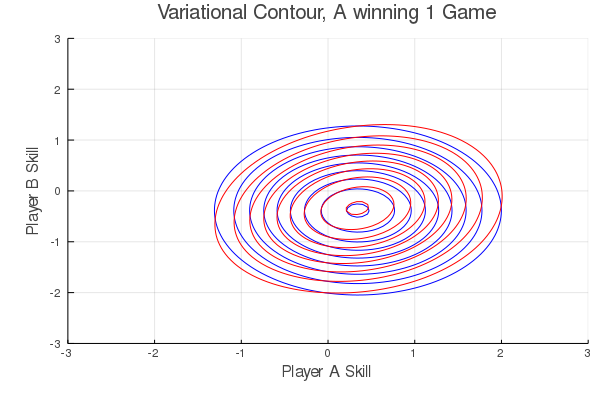
\includegraphics[width=12cm,keepaspectratio]{plots/variational_fit_A1_B0.png}
\end{figure}

Final loss: 0.73
\pagebreak

  \item {\bf [2 points]} Initialize a variational distribution parameters and optimize them to approximate the joint
    where we observe player A winning 10 games.
    Report the final loss.
    Also plot the optimized variational approximation contours (in blue) aand the target distribution (in red) on the same axes.

\begin{verbatim}
evidence = two_player_toy_games(10,0)
params_learned = fit_toy_variational_dist(toy_params_init, evidence, num_itrs=700)

p = plot(title="Variational Contour, A winning 10 Games",
    xlabel = "Player A Skill",
    ylabel = "Player B Skill")
skillcontour!(zs -> exp(factorized_gaussian_log_density(params_learned[1],params_learned[2],zs)),colour=:blue)
skillcontour!(zs -> exp(joint_log_density(zs, evidence)),colour=:red)
display(p);
savefig(joinpath("plots","variational_fit_A10_B0.png"))
\end{verbatim}

\begin{figure}[h]
  \centering
  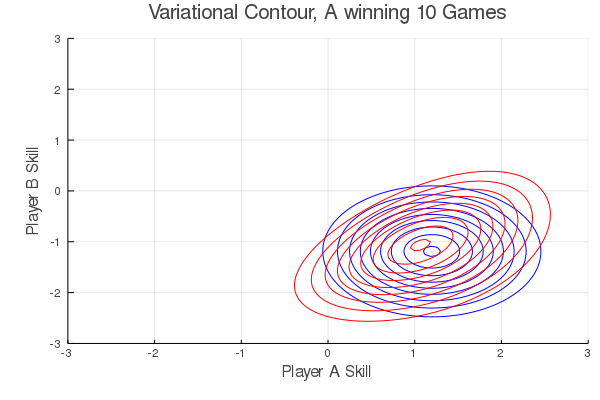
\includegraphics[width=12cm,keepaspectratio]{plots/variational_fit_A10_B0.png}
\end{figure}

Final loss: 2.93

\pagebreak
    
  \item {\bf [2 points]} Initialize a variational distribution parameters and optimize them to approximate the joint
    where we observe player A winning 10 games and player B winning 10 games.
    Report the final loss.
    Also plot the optimized variational approximation contours (in blue) aand the target distribution (in red) on the same axes.
\end{enumerate}
For all plots, label both axes.

\begin{verbatim}
evidence = two_player_toy_games(10,10)
params_learned = fit_toy_variational_dist(toy_params_init, evidence, num_itrs=700)

p = plot(title="Variational Contour, A winning 10 Games, B wining 10 Games ",
    xlabel = "Player A Skill",
    ylabel = "Player B Skill")
skillcontour!(zs -> exp(factorized_gaussian_log_density(params_learned[1],params_learned[2],zs)),colour=:blue)
skillcontour!(zs -> exp(joint_log_density(zs, evidence)),colour=:red)
display(p);
savefig(joinpath("plots","variational_fit_A10_B10.png"))
\end{verbatim}

\begin{figure}[h]
  \centering
  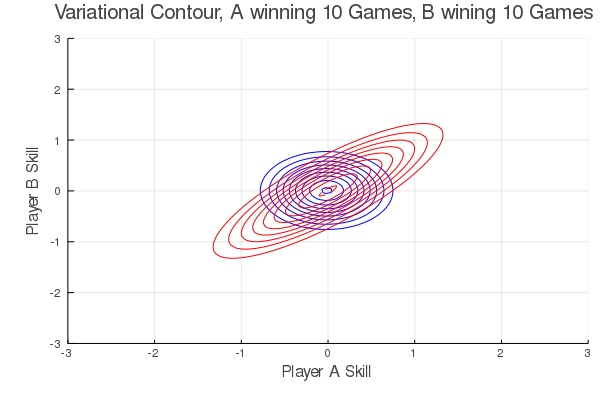
\includegraphics[width=12cm,keepaspectratio]{plots/variational_fit_A10_B10.png}
\end{figure}

Final loss: 15.67

\pagebreak
\section{Approximate inference conditioned on real data [24 points]}
Load the dataset from \texttt{tennis\_data.mat} containing two matrices:

\begin{itemize}
	\item W is a 107 by 1 matrix, whose $i$’th entry is the name of player $i$.
	\item G is a 1801 by 2 matrix of game outcomes (actually tennis matches), one row per game.
The first column contains the indices of the players who won.
The second column contains the indices of the player who lost.
\end{itemize}

Compute the following using your code from the earlier questions in the assignment, but conditioning on the tennis match outcomes:
\begin{enumerate}[label=(\alph*)]
\item {\bf [1 point]} For any two players $i$ and $j$, $p(z_i, z_j | \textnormal{all games})$ is always proportional to
	$p(z_i, z_j , \textnormal{all games})$.
	In general, are the isocontours of $p(z_i, z_j | \textnormal{all games})$ the same as those of
	$p(z_i, z_j | \textnormal{games between $i$ and $j$})$?  That is, do the games between
	other players besides $i$ and $j$ provide information about the skill of
	players $i$ and $j$?  A simple yes or no suffices.
	
	Hint: One way to answer this is to draw the graphical model for three players,
	$i$, $j$, and $k$, and the results of games between all three pairs, and then
	examine conditional independencies.  If you do this, there's no need to include
	the graphical models in your assignment.

        Yes.
        \pagebreak
\item {\bf [5 points]} Write a new optimization function \texttt{fit\_variational\_dist} like the one from the 
  previous question except it does not plot anything.
  Initialize a variational distribution and fit it to the joint distribution with all the observed tennis games from the dataset.
  Report the final negative ELBO estimate after optimization.

\begin{verbatim}
using MAT
vars = matread("tennis_data.mat")
player_names = vars["W"]
tennis_games = Int.(vars["G"])
num_players = length(player_names)
print("Loaded data for $num_players players")

function fit_variational_dist(init_params,
                              tennis_games;
                              num_itrs=200,
                              lr= 1e-2,
                              num_q_samples = 10)
  params_cur = init_params
  for i in 1:num_itrs

    grad_params = gradient(in -> neg_toy_elbo(in,
                                              games=tennis_games;
                                              num_samples=num_q_samples)[1],
                          params_cur)[1]
    params_cur =  params_cur .- lr .* grad_params;

    if i % 25 == 0 || i == num_itrs
      neg_elbo = neg_toy_elbo(params_cur,
                              games=tennis_games;
                              num_samples=num_q_samples)[1]
      @info "neg_elbo: " neg_elbo
    end
  end
  neg_elbo = neg_toy_elbo(params_cur,
                          games=tennis_games;
                          num_samples=num_q_samples)[1]
  @info "neg_elbo: " neg_elbo
  return params_cur
end

init_mu = randn(num_players)
init_log_sigma = rand(Uniform(0,1), num_players)
init_params = (init_mu, init_log_sigma)

# Train variational distribution
trained_params = fit_variational_dist(init_params,
                                      tennis_games,
                                      num_itrs=700,
                                      lr= 5e-3,
                                      num_q_samples = 30)
\end{verbatim}
  
  negative ELBO estimate: 1142.91

  \pagebreak
  
\item {\bf [2 points]} Plot the approximate mean and variance of all players, sorted by skill.  For example, in Julia, you can use:
\texttt{perm = sortperm(means);
	plot(means[perm], yerror=exp.(logstd[perm]))}
      There's no need to include the names of the players.

\begin{verbatim}
perm = sortperm(trained_params[1])
plot(trained_params[1][perm], yerror=exp.(trained_params[2][perm]),
    title="Player Skills and Uncertainty(S.D.)",
    xlabel = "Player Enumeration",
    ylabel = "Player Skill",
    legend=false)
savefig(joinpath("plots","4c_all_player_skills.png"))
\end{verbatim}

\begin{figure}[h]
  \centering
  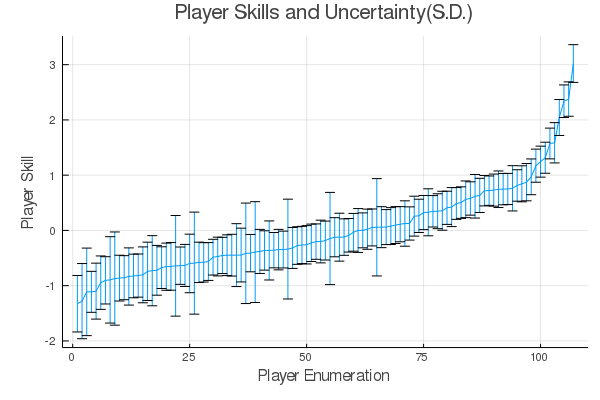
\includegraphics[width=12cm,keepaspectratio]{plots/4c_all_player_skills.png}
\end{figure}

\item {\bf [2 points]} List the names of the 10 players with the highest mean skill under the variational model.

\begin{verbatim}
idx_ordered = sortperm(trained_params[1])
idx_top = reverse(idx_ordered[end-9:end])
top_players = player_names[idx_top]

top_players_skills = trained_params[1][idx_top]
top = collect(zip(top_players,top_players_skills))
print("top players: ", top)
\end{verbatim}

  \begin{tabular}{|c|c|c|}
    \hline
    1&Novak-Djokovic& 3.020\\
    \hline
    2&Roger-Federer& 2.377\\
    \hline
    3&Rafael-Nadal& 2.338\\
    \hline
    4&Andy-Murray& 2.043\\
    \hline
    5&Robin-Soderling& 1.586\\
    \hline
    6&David-Ferrer& 1.573\\
    \hline
    7&Jo-Wilfried-Tsonga& 1.315\\
    \hline
    8&Tomas-Berdych& 1.244\\
    \hline
    9&Juan-Martin-Del-Potro& 1.172\\
    \hline
    10&Richard-Gasquet& 0.970\\
    \hline
  \end{tabular}

  
\item {\bf [3 points]} Plot the joint posterior over the skills of Roger Federer and Rafael Nadal.

\begin{verbatim}
idx_1 = findall(x-> x =="Roger-Federer", player_names)
idx_2 = findall(x-> x == "Rafael-Nadal", player_names)
idx = [idx_1;idx_2]
m = trained_params[1][idx]
ls = trained_params[2][idx]

p = plot(title="Joint Posterior Plot",
    xlabel = "Roger-Federer Skill",
    ylabel = "Rafael-Nadal Skill")
skillcontour!(zs -> exp(factorized_gaussian_log_density(m,ls,zs)))
display(p);
savefig(joinpath("plots","joint_posterior_federer_nadal.png"))
\end{verbatim}

\begin{figure}[h]
  \centering
  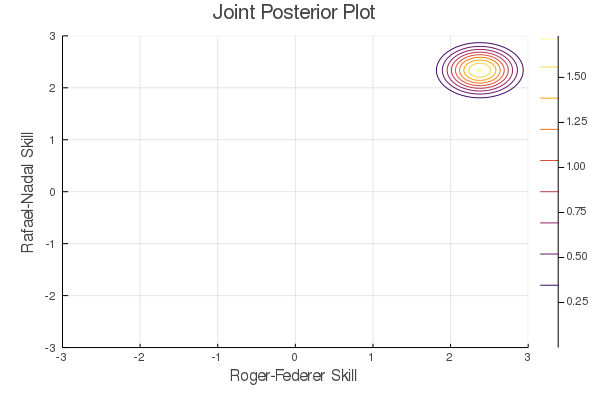
\includegraphics[width=12cm,keepaspectratio]{plots/joint_posterior_federer_nadal.png}
\end{figure}

\pagebreak

\item {\bf [5 points]} Derive the exact probability under a factorized Guassian over two players' skills that one has higher skill than the other, as a function of the two means and variances over their skills.
\begin{itemize}
\item Hint 1: Use a linear change of variables $y_A, y_B = z_A - z_B, z_B$.  What does the line of equal skill look like after this transformation?
\item Hint 2: If $X \sim \mathcal{N}(\mu, \Sigma)$, then $AX \sim \mathcal{N}(A \mu, A^{T} \Sigma A)$ where $A$ is a linear transformation.
\item Hint 3: Marginalization in Gaussians is easy: if $X \sim \mathcal{N}(\mu, \Sigma)$, then the $i$th element of $X$ has a marginal distribution $X_i \sim \mathcal{N}(\mu_i, \Sigma_{ii})$

  \begin{align*}
    let\ y_a &= z_a-z_b\\
    let\ y_b &= z_b\\
    p(z_a>z_b) & = p(z_a-z_b>0) = p(y_a>0)\\
    p(y_b) &= p(z_b)\\
    y & =
        \begin{bmatrix}
          y_a\\y_b
        \end{bmatrix}\\
    z & =
        \begin{bmatrix}
          z_a\\z_b
        \end{bmatrix}\\
    y & = Az, A =
        \begin{bmatrix}
          1 & -1\\ 0 & 1
        \end{bmatrix}\\
    \bar{y} &= A\bar{z}\\
    \Sigma_y &= A^T\Sigma_z A\\
    \bar{y} &=
    \begin{bmatrix}
      \mu_a-\mu_b\\
      \mu_b
    \end{bmatrix}\\
    \Sigma_y &=
               \begin{bmatrix}
                 1 & -1\\ 0 & 1
               \end{bmatrix}^T 
    \begin{bmatrix}
      \sigma_a^2 & 0 \\ 0 & \sigma_b^2
    \end{bmatrix}
    \begin{bmatrix}
      1 & -1\\ 0 & 1
    \end{bmatrix} =
                   \begin{bmatrix}
                     \sigma_a^2 & -\sigma_a^2\\
                     -\sigma_a^2 & \sigma_a^2 + \sigma_b^2\\
                   \end{bmatrix}\\
    p(y_a) &= \int_{x} p(y_a,y_b=x) dx\\
             &\text{marginalize over gaussian: }\\
    p(y_a) &\sim \N(\mu_a-\mu_b,\sigma_a^2)\\
    p(y_a>0)&=1-\int_{-\infty}^0 p(y_a=x)dx\\
    z_{score} &= \frac{x-(\mu_a-\mu_b)}{\sigma_a}\bigg|_{x=0}\\
    \int_{-\infty}^0 p(y_a=x)dx &= \Phi(z_{score})\\
    p(y_a>0)&=1-\Phi(z_{score}),\ \Phi(z_{score}) = \int_{-\infty}^{z_{score}} \frac{1}{\sqrt{2\pi}} e^{-\frac{1}{2}t^2}dt,\ z_{score} = \frac{x-(\mu_a-\mu_b)}{\sigma_a}\bigg|_{x=0}\\\\
  \end{align*}
  \pagebreak
\end{itemize}
\item {\bf [2 points]} Compute the probability under your approximate posterior that
	Roger Federer has higher skill than Rafael Nadal.
	Compute this quantity exactly, and then estimate it using simple Monte Carlo with 10000 examples.\\
        Exact:
        \begin{align*}
          let\ z_a &= skill_{Roger\ Federer}\\
          let\ z_b &= skill_{Rafael\ Nadal}\\
          z_{score} &= \frac{x-(\mu_a-\mu_b)}{\sigma_a}\bigg|_{x=0}=-0.124715\\
          p(z_a>z_b)&=1-\Phi(z_{score}),\ \Phi(z_{score}) = \int_{-\infty}^{z_{score}} \frac{1}{\sqrt{2\pi}} e^{-\frac{1}{2}t^2}dt\\
                   & = 0.5496
        \end{align*}
        Monte Carlo Estimation:
        \begin{align*}
          N&=10000\\
          q(z_a|x) &= \N(\mu_a, var=\sigma_a^2),\ q(z_b|x) = \N(\mu_b, var=\sigma_b^2)\\
          p(z_a > z_b) &\approx \frac{1}{N} \sum_{i=1}^{N} [I(a>b) : a \sim q(z_a|x), b \sim q(z_b|x)] = 0.546
        \end{align*}
\begin{verbatim}
#exact prob of skill_federer > skill_nadal from learned posterior
idx_nadal = findall(x-> x == "Rafael-Nadal", player_names)[1]
idx_federer = findall(x-> x =="Roger-Federer", player_names)[1]
m_federer = trained_params[1][idx_federer]
ls_federer = trained_params[2][idx_federer]
m_nadal = trained_params[1][idx_nadal]
ls_nadal = trained_params[2][idx_nadal]
z_score = (0-(m_federer-m_nadal))/exp(ls_federer)
p_exact = 1-cdf(Normal(0, 1), z_score) 
#monte carlo for federer vs nadal
n=10000
sample_federer = randn(1,1000) .* exp(ls_federer) .+ m_federer
sample_last = randn(1,1000) .* exp(ls_nadal) .+ m_nadal
indicator = sample_federer .> sample_last
mean(indicator)
\end{verbatim}

        \begin{figure}[h]
  \centering
  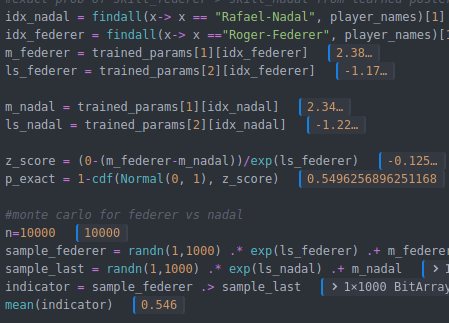
\includegraphics[width=8cm,keepaspectratio]{plots/skill_federer_vs_nadal.png}
\end{figure}

        \pagebreak
        
\item {\bf [2 points]} Compute the probability that Roger Federer is better than the player
	with the lowest mean skill.
	Compute this quantity exactly, and then estimate it using simple Monte Carlo with 10000 examples.
        Exact:
        \begin{align*}
          let\ z_a &= skill_{Roger\ Federer}\\
          let\ z_b &= skill_{Lowest Rank}\\
          z_{score} &= \frac{x-(\mu_a-\mu_b)}{\sigma_a}\bigg|_{x=0}=-11.90362\\
          p(z_a>z_b)&=1-\Phi(z_{score}),\ \Phi(z_{score}) = \int_{-\infty}^{z_{score}} \frac{1}{\sqrt{2\pi}} e^{-\frac{1}{2}t^2}dt\\
                   &\approx 1
        \end{align*}
        Monte Carlo Estimation:
        \begin{align*}
          N&=10000\\
          q(z_a|x) &= \N(\mu_a, var=\sigma_a^2),\ q(z_b|x) = \N(\mu_b, var=\sigma_b^2)\\
          p(z_a > z_b) &\approx \frac{1}{N} \sum_{i=1}^{N} [I(a>b) : a \sim q(z_a|x), b \sim q(z_b|x)]=1
        \end{align*}

\begin{verbatim}
#exact prob of skill_federer > skill_last_ranked from learned posterior
idx_ordered = sortperm(trained_params[1])
idx_last = idx_ordered[1]
last_player = player_names[idx_last]
m_last = trained_params[1][idx_last]
ls_last = trained_params[2][idx_last]
idx_federer = findall(x-> x =="Roger-Federer", player_names)[1]
m_federer = trained_params[1][idx_federer]
ls_federer = trained_params[2][idx_federer]
z_score = (0-(m_federer-m_last))/exp(ls_federer)
p_exact = 1-cdf(Normal(0, 1), z_score)
#monte carlo for federer vs last ranked player
n=10000
sample_federer = randn(1,1000) .* exp(ls_federer) .+ m_federer
sample_last = randn(1,1000) .* exp(ls_last) .+ m_last
indicator = sample_federer .> sample_last
mean(indicator)
\end{verbatim}

        \begin{figure}[h]
  \centering
  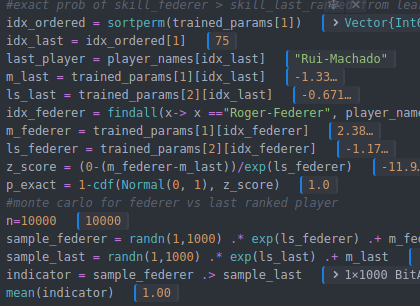
\includegraphics[width=8cm,keepaspectratio]{plots/skill_federer_vs_last.png}
\end{figure}

        \pagebreak
        
\item {\bf [2 points]} Imagine that we knew ahead of time that we were examining the
	skills of top tennis players, and so changed our prior on all players to
	Normal(10, 1).
	Which answers in this section would this change?
	No need to show your work, just list the letters of the questions whose answers would be different in expectation.\\
        
        No change, under the assumption that player skill is single modal and thus using single modal gaussian for prior and posterior allows optimization convergence to near a same global minimal. This can also be confirmed from different initialization of prior parameters.
\end{enumerate}

\end{document}
